\section {The arduino components}
\begin {frame} {Outline}
    \tableofcontents [current]
\end{frame}

\begin{frame}{The arduino components}
	\begin{center}
		% let me show to you a starter kit for arduino
		\includegraphics<1> [width=1.0\textwidth,keepaspectratio] {img/components}
		\includegraphics<2> [width=1\textwidth,keepaspectratio] {img/components_resistors.jpg}
		\includegraphics<3> [width=1\textwidth,keepaspectratio] {img/components_leds.jpg}
		\includegraphics<4> [width=1\textwidth,keepaspectratio] {img/components_light_sensor.jpg}
		\includegraphics<5> [width=1\textwidth,keepaspectratio] {img/components_pushbuttons.jpg}
		\includegraphics<6> [width=1\textwidth,keepaspectratio] {img/components_breadboard.jpg}
		\includegraphics<7> [width=1\textwidth,keepaspectratio] {img/components_wires.jpg}
		\includegraphics<8> [width=1\textwidth,keepaspectratio] {img/components_potentiometers.jpg}
	\end{center}
\end{frame}

\begin{frame}{The shields}
	\begin{itemize}
		\item Ethernet (36-75\$) / WiFi (10-70\$) / GPS (50-110\$) / Wave (4.5-30\$)
		\item Sensors (temperature, humidity, luminosity)
		\item NFC / RFID / SD card
		\item LCD
		\item …
		% There is no real limit, you just do whatever you can do with the power supplied by arduino
	\end{itemize}
\end{frame}

\begin{frame}{Stacked shields}
	\begin{center}
		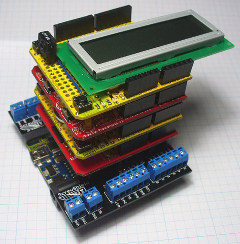
\includegraphics [width=0.5\textwidth,keepaspectratio] {img/stacked-shields}
	\end{center}
\end{frame}

%%%% TODO : add images
